%!TEX root = ../main.tex

\section{Energy calibration of the MCS analyser}
\label{sec:ecal}

As described in \autoref{sec:mössbauer-spectroscopy}, Mössbauer spectroscopy does not
rely on an extremely precise measurement of the photon energy. Due to resonant
absorption it is sufficient to merely count the number of photons transmitted through
an absorber to gather information about its atomic energy levels and existing nuclear
transitions. However, in order to allow for more detailed analysis in the following
evaluation the relative difference of transition energies needs to be quantified.
For this purpose as well as a proof of concept, The $\gamma$-spectrum of $^{57}$Co is
measured. Visible in the observed spectrum in \autoref{fig:ecal} is a characteristic
Lorentzian peak that reperesents the \SI{14.4}{\kilo\electronvolt} resonance of the 
excited $^{57}$Fe$^{*}$ state. The exact fitfunction as well as fit results are given
in the below \autoref{eq:ecal-fit}

\begin{equation}
\label{eq:ecal-fit}
f(\mathcal{C}) = \frac{A}{(\mathcal{C}^2-\omega_0^2)^2 + \gamma^2\omega_0^2}
\end{equation}

\begin{align*}
	A &= \SI{8.68\pm 0.36e+10}{} \\
	\omega_0 &= \SI{67.84\pm 0.08}{} \\
	\gamma &= \SI{23.25\pm 0.52}{}
\end{align*}

\begin{equation*}
\text{COV}(A,\omega_0,\gamma) =
\left[
\begin{array}{c c c}
	1.28\times10^{19} & 1.00\times10^{7} & 1.86\times10^{9} \\
	1.00\times10^{7} & 5.66\times10^{-3} & -6.41\times10^{-4} \\
	1.86\times10^{9} & -6.41\times10^{-4} & 2.75\times10^{-1}
\end{array}
\right]
\end{equation*}

\begin{equation*}
	\Delta f(\mathcal{C}) = \sqrt{ (\nabla f(\mathcal{C}))^T\;\text{COV}(A,\omega_0,\gamma)\;\nabla f(\mathcal{C})}
\end{equation*}

\begin{figure}
	\centering
	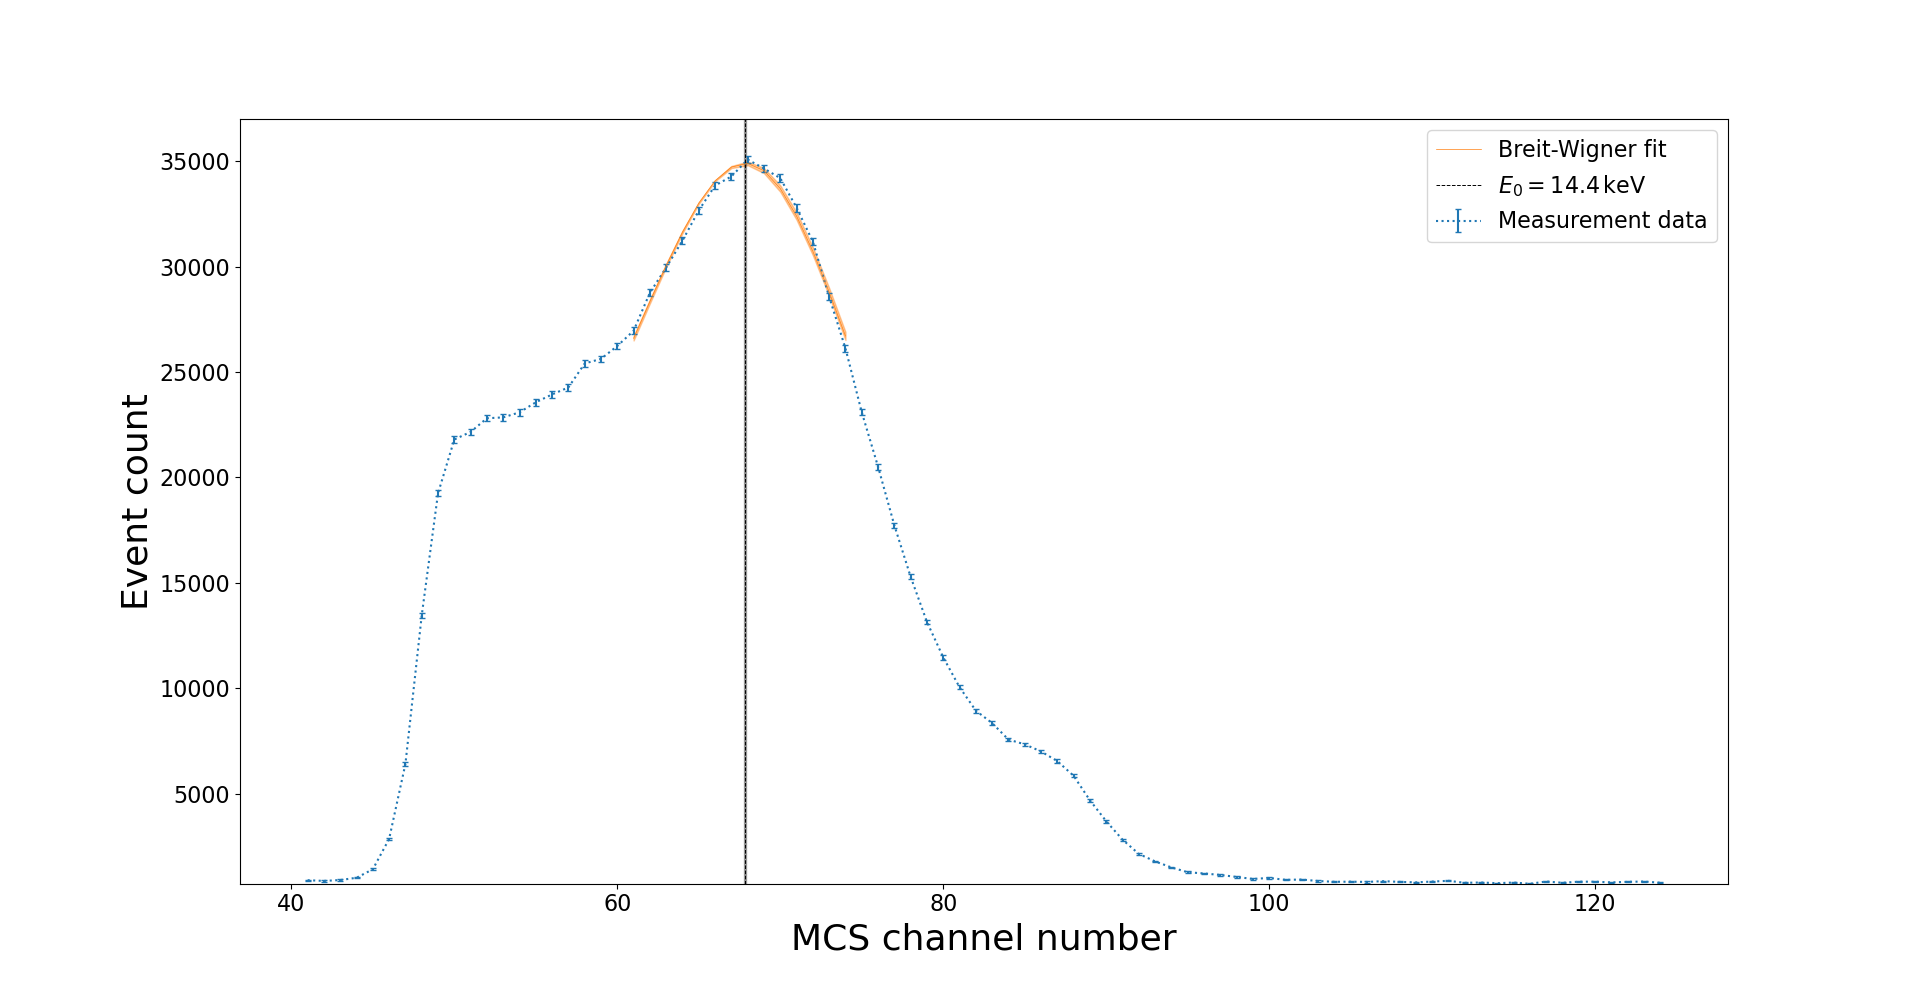
\includegraphics[width=1.0\textwidth]{./fig/calibration.png}
	\caption{The error on the measured counts is assumed to be Poissonian.
	Because the amplitude $A$ does not hold physical information other than the 
	flux of the $\gamma$-source, uncertainties and correlations in $A$ are
	neglected in the below error propagation.}
	\label{fig:ecal}
\end{figure}
